%%%%%%%%%%%%
%
% $Autor: Wings $
% $Datum: 2019-03-05 08:03:15Z $
% $Pfad: TemplateSensor $
% $Version: 4250 $
% !TeX spellcheck = en_GB/de_DE
% !TeX encoding = utf8
% !TeX root = filename 
% !TeX TXS-program:bibliography = txs:///biber
%
%%%%%%%%%%%%

% Structure
\chapter{MikroTik LR8 Kit Gateway}
	Dieses Kapitel beschreibt Aufbau, Funktionsweise und Konfiguration des MikroTik LR8 Kit Gateways. Es erläutert die Hardwarestruktur bestehend aus der Routerplattform RBwAPR-2nD und der LoRaWAN-Erweiterungskarte R11e-LR8, einschließlich mechanischem Aufbau, Antennenkonzept und verfügbaren Schnittstellen. Ergänzend werden technische Daten der Komponenten dargestellt. Anschließend folgt eine detaillierte Anleitung zur Inbetriebnahme, einschließlich Stromversorgung, Antennenanschluss, Ersteinrichtung und der Anbindung an einen \ac{lorawan} Network Server. Die beschriebenen Schritte ermöglichen den vollständigen praktischen Einsatz des Gateways in einer privaten oder öffentlichen \ac{lorawan}-Infrastruktur.

\section{Einleitung}
	MikroTik LR8 Kit Gateway ist ein vollständiges LoRaWAN-Gateway, das über \textbf{acht parallele Kanäle} verfügt. Laut Mikrotik funktioniert es \emph{out of the box} und besitzt einen vorinstallierten UDP-Packet-Forwarder, der sowohl zu öffentlichen als auch zu privaten LoRaWAN-Netzwerkservern eine Verbindung herstellen kann. Das wetterfeste Gehäuse ermöglicht den Einsatz im Au{\ss}enbereich. Zusätzlich bietet das Gerät einen kabelgebundenen Ethernet-Anschluss sowie einen 2.4 GHz WLAN Access Point \cite{mikrotik:2020}.
	
	Das Gateway besteht im Wesentlichen aus zwei Komponenten:
	\begin{itemize}
		\item \textbf{RBwAPR-2nD} – eine universelle Routerplattform, die das „Gehirn“ des Systems bildet. Sie verfügt über eine Netzwerkschnittstelle, eine CPU, WLAN sowie einen Mini-PCIe-Steckplatz zum Anschluss von Erweiterungskarten.
		\item \textbf{R11e-LR8} – eine Erweiterungskarte, welche die LoRaWAN-Funktionalität bereitstellt. Die Karte basiert auf einem Semtech-Konzentratorchip (SX1301) und unterstützt den gleichzeitigen Empfang von bis zu \textbf{acht LoRa-Kanälen}. Dadurch können mehrere Endgeräte auf unterschiedlichen Frequenzen und Spreading Factors parallel empfangen werden. Die Karte übernimmt sowohl das Senden von LoRa-Nachrichten gemä{\ss} den Befehlen des Routers als auch den Empfang eingehender Pakete. Diese werden demoduliert und anschlie{\ss}end an das entsprechende RouterOS-Modul weitergeleitet, welches die weitere Verarbeitung und die Übermittlung an den LoRaWAN-Netzwerkserver übernimmt \cite{mikrotik:2020} \cite{mikrotik:2024}.
	\end{itemize}

	\begin{figure}[H]
		\centering
		\begin{tikzpicture}
			\mikrotikGatewayTopEnclosure{0.5}{0}{0}{0}
			\mikrotikGatewayBottomEnclosure{0.5}{0}{0}{0}
			
		\end{tikzpicture}
		\caption{Frontansicht des MikroTik wAP LR8 Gateways \cite{mikrotik:2020}}
	\end{figure}
	
\section{Aufbau des Gateways}
	\subsection{RBwAPR-2nD (Routerplattform)}
		Der RBwAPR-2nD bildet die zentrale Routerplattform des Gateways und stellt sämtliche Netzwerk- und Systemfunktionen bereit, die für den Betrieb eines LoRaWAN-Gateways erforderlich sind. Dazu gehören ein integrierter 2.4-GHz-WLAN-Access Point, ein Ethernet-Port sowie eine CPU mit RouterOS als Betriebssystem. Über den vorhandenen Mini-PCIe-Steckplatz kann der Router um zusätzliche Module wie LoRaWAN- oder LTE-Erweiterungskarten ergänzt werden. In der hier beschriebenen Konfiguration ist in diesem Steckplatz die LoRa-Erweiterungskarte eingesetzt. Da jedoch lediglich ein einziger Mini-PCIe-Port zur Verfügung steht, kann immer nur ein Modul gleichzeitig betrieben werden. Die Plattform übernimmt die Verarbeitung und Weiterleitung der von der LoRa-Karte empfangenen Pakete und kommuniziert über das Netzwerk mithilfe des von MikroTik bereitgestellten UDP-Packet-Forwarders mit einem LoRaWAN-Server wie ChirpStack oder The Things Stack \cite{mikrotik:2020}.
		
		\begin{figure}[H]
			\centering
			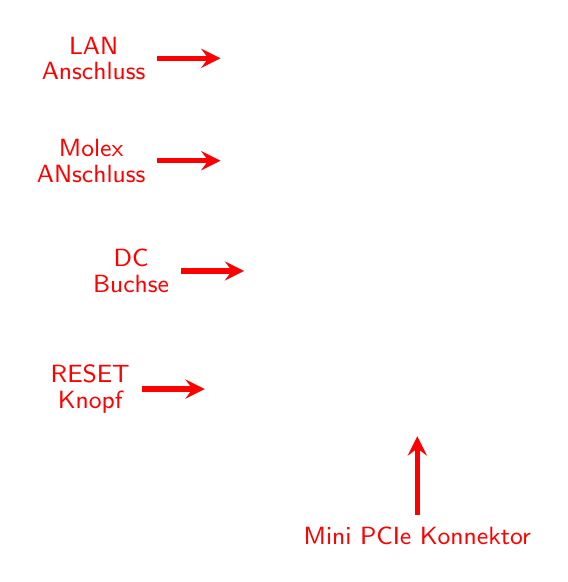
\begin{tikzpicture}
				\tikzset{
					textDef/.style={font=\sffamily\small,},
					lineScaled/.style={line width={2pt}},
					arrowStyle/.style={lineScaled, >=stealth, red},
				}
				\routerPlatform{0.8}{0}{0}{0}
				
				\draw[arrowStyle, <-] (-3.5, 2.3) -- ++(-0.8,0) node[left, textDef]{\shortstack{LAN\\Anschluss}};
				\draw[arrowStyle, <-] (-3.5, 1) -- ++(-0.8,0) node[left, textDef]{\shortstack{Molex \\ ANschluss}};
				\draw[arrowStyle, <-] (-3.2, -0.4) -- ++(-0.8,0) node[left, textDef]{\shortstack{DC\\ Buchse}};
				\draw[arrowStyle, <-] (-3.7, -1.9) -- ++(-0.8,0) node[left, textDef]{\shortstack{RESET\\Knopf}};
				\draw[arrowStyle, <-] (-1, -2.5) -- ++(0,-1) node[below, textDef]{\shortstack{Mini PCIe Konnektor}};
			\end{tikzpicture}
			\caption{Routerplattform RBwAPR-2nD}
		\end{figure}
		
	\subsection{R11e-LR8 (LoRaWAN-Erweiterungskarte)}
		Die R11e-LR8 ist eine Mini-PCIe-Erweiterungskarte, die die gesamte LoRaWAN-Funkfunktionalität bereitstellt. Sie basiert auf dem Semtech-Konzentratorchip SX1301 und unterstützt den gleichzeitigen Empfang von bis zu acht Kanälen auf verschiedenen Frequenzen und Spreading Factors. Die Karte demoduliert eingehende LoRa-Pakete und übergibt sie an RouterOS zur weiteren Verarbeitung und Weiterleitung an den Netzwerkserver. Umgekehrt sendet sie LoRa-Nachrichten entsprechend der vom Router bereitgestellten Befehle. Über ein u.FL-Anschluss wird die externe oder interne Antenne angeschlossen \cite{mikrotik:2024}.
		
		\begin{figure}[H]
			\centering
			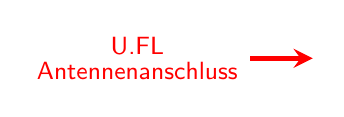
\begin{tikzpicture}
				\tikzset{
					textDef/.style={font=\sffamily\small,},
					lineScaled/.style={line width={2pt}},
					arrowStyle/.style={lineScaled, >=stealth, red},
				}
				\loraCard{0.8}{90}{0}{0}
				
				\draw[arrowStyle, <-] (-2, 0.1) -- ++(-0.8,0) node[left, textDef]{\shortstack{U.FL\\Antennenanschluss}};
			\end{tikzpicture}
			\caption{LoRaWAN-Erweiterungskarte R11e-LR8}
		\end{figure}
		
		Die Erweiterungskarte kann nicht unabhängig betrieben werden und wird über den Mini-PCIe-Steckplatz mit der Routerplattform verbunden.
		
		\begin{figure}[H]
			\centering
			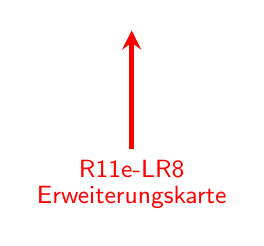
\begin{tikzpicture}
				\tikzset{
					textDef/.style={font=\sffamily\small,},
					lineScaled/.style={line width={2pt}},
					arrowStyle/.style={lineScaled, >=stealth, red},
				}
				\routerPlatform{1}{0}{0}{0}
				\loraCard{1}{0}{0}{0}
				
				
				\draw[arrowStyle, <-] (-1, -2.5) -- ++(0,-1.5) node[below, textDef]{\shortstack{R11e-LR8\\Erweiterungskarte}};
			\end{tikzpicture}
			\caption{R11e-LR8 im Mini-PCIe-Steckplatz der Routerplattform}
		\end{figure}
		
	\subsection{Gehäuse und mechanischer Aufbau}
		Das wAP-Gehäuse ist für den Einsatz im Au{\ss}enbereich ausgelegt und erfüllt die Anforderungen an eine robuste und wetterfeste Installation. Es besteht aus einem widerstandsfähigen Kunststoffmaterial mit abgedichteten Öffnungen und einer verschraubten Unterseite, um den Schutz gegen Feuchtigkeit und Staub sicherzustellen. Die interne Montagestruktur nimmt sowohl die Routerplattform als auch die LoRa-Karte sicher auf und ermöglicht gleichzeitig eine saubere Führung der Antennenkabel. Das kompakte Formfaktor sowie die flache Bauform erleichtern die Montage an Wänden, Masten oder Au{\ss}enfassaden \cite{mikrotik:2020}.
		
		\begin{figure}[H]
			\centering
			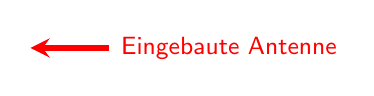
\begin{tikzpicture}
				\tikzset{
					textDef/.style={font=\sffamily\small,},
					lineScaled/.style={line width={2pt}},
					arrowStyle/.style={lineScaled, >=stealth, red},
				}
				\mikrotikInside
				
				
				\draw[arrowStyle, <-] (3.5, -2) -- ++(1,0) node[right, textDef]{\shortstack{Eingebaute Antenne}};
			\end{tikzpicture}
			\caption{Innerer Aufbau des Gateways}
		\end{figure}


\section{Technische Daten}
	\subsection{Router}
		\begin{table}[H]
			\centering
			\begin{tabular}{| l | l |}
				\hline
				Produktcode & RBwAPR-2nD \\
				\hline
				Architektur & MIPSBE \\
				\hline
				CPU & QCA9531, 1 Kern, 650 MHz \\
				\hline
				RAM & 64 MB \\
				\hline
				Flash-Speicher & 16 MB \\
				\hline
				Betriebssystem & RouterOS\\
				\hline
				Mittlere Zeit zwischen Ausfällen & ca. 100\,000 h bei \(25^\circ\mathrm{C}\) \\
				\hline
				Temperaturbereich & \(-40^\circ\mathrm{C}\) bis \(60^\circ\mathrm{C}\) \\
				\hline
				Kühlung & Passiv \\
				\hline
			\end{tabular}
			\caption{Technische Daten – Routerplattform RBwAPR-2nD \cite{mikrotik:2020}}
		\end{table}
		
	\subsection{LoRaWAN-Karte}
		\begin{table}[H]
			\centering
			\begin{tabular}{| l | l |}
				\hline
				Produktcode & R11e-LR8 \\
				\hline
				Frequenzbereich & 863--870 MHz (EU-Band) \\
				\hline
				Konzentratorchip & Semtech SX1301 \\
				\hline
				Kanäle & 8 parallele LoRa-Kanäle \\
				\hline
				Modulationsarten & LoRa, FSK \\
				\hline
				Antennenanschluss & u.FL-Anschluss \\
				\hline
				Schnittstelle & Mini-PCIe \\
				\hline
				Unterstützte Klassen & Klasse A und Klasse C \\
				\hline
				RF-Ausgangsleistung & bis zu 27 dBm, in der EU auf 14 dBm begrenzt \\
				\hline
				Maximale Empfangsempfindlichkeit & bis zu –137 dBm bei SF12 (abhängig von der Antenne) \\
				\hline
				Leistungsaufnahme & 2 W \\
				\hline
				Betriebstemperaturbereich & \(-40^\circ\mathrm{C}\) bis \(70^\circ\mathrm{C}\) \\
				\hline
			\end{tabular}
			\caption{Technische Daten – LoRaWAN-Erweiterungskarte R11e-LR8 \cite{mikrotik:2020}, \cite{mikrotik:2024}}
		\end{table}
		
		
		
	\subsection{Antenne}
		\begin{table}[H]
			\centering
			\begin{tabular}{| l | l |}
				\hline
				Interne Antenne & 2 dBi  \\
				\hline
				Externe Antenne & Unterstützt (über u.FL Anschluss) \\
				\hline
			\end{tabular}
			\caption{Technische Daten – Antenne \cite{mikrotik:2020}}
		\end{table}
		
	\subsection{Anschlüsse}
		\begin{table}[H]
			\centering
			\begin{tabular}{| l | l |}
				\hline
				Ethernet & 1 \(\times\) 10/100 Mbit/s \\
				\hline
				Mini-PCIe & 1 Slot (LoRa oder LTE) \\
				\hline
				SIM-Slot & 1 \(\times\) Mini-SIM (nur mit LTE-Modem nutzbar) \\
				\hline
				DC-Eingänge & 9 - 30 V (DC Jack, Automotive, PoE-IN) \\
				\hline
				PoE-IN & Passives PoE, 9 - 30 V \\
				\hline
				IP-Schutzklasse & IP54 \\
				\hline
			\end{tabular}
			\caption{Technische Daten – Anschlüsse und Schnittstellen \cite{mikrotik:2020}}
		\end{table}
		
		\begin{figure}[H]
			\centering
			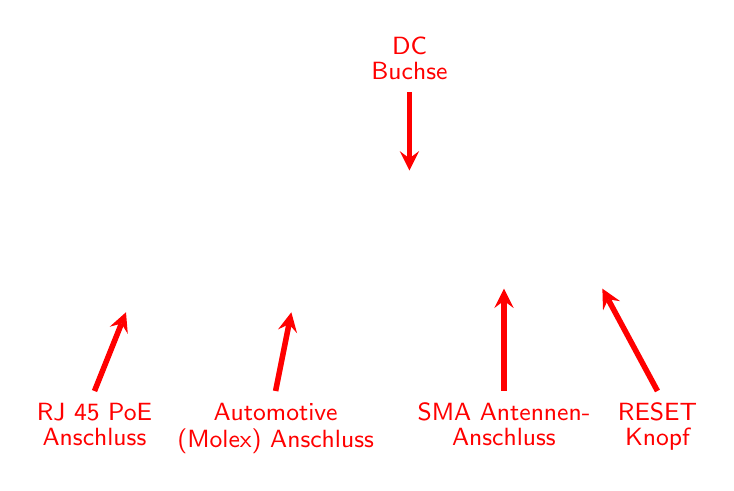
\begin{tikzpicture}
				\tikzset{
					textDef/.style={font=\sffamily\small,},
					lineScaled/.style={line width={2pt}},
					arrowStyle/.style={lineScaled, >=stealth, red},
				}
				\gatewayConnectors
				
				
				
				\draw[arrowStyle, <-] (-3.1, -0.8) -- ++(-0.4, -1) node[below, textDef]{\shortstack{RJ 45 PoE\\ Anschluss}};
				\draw[arrowStyle, <-] (-1, -0.8) -- ++(-0.2, -1) node[below, textDef]{\shortstack{Automotive\\(Molex) Anschluss}};
				\draw[arrowStyle, <-] (1.7, -0.5) -- ++(0, -1.3) node[below, textDef]{\shortstack{SMA Antennen-\\Anschluss}};
				\draw[arrowStyle, <-] (2.95, -0.5) -- ++(0.7, -1.3) node[below, textDef]{\shortstack{RESET\\Knopf}};
				\draw[arrowStyle, <-] (0.5, 1) -- ++(0, 1) node[above, textDef]{\shortstack{DC\\Buchse}};
			\end{tikzpicture}
			\caption{Übersicht der verfügbaren Anschlüsse des Gateways}
		\end{figure}

\section{Stromversorgung}
	\subsection{PoE}
	PoE versorgt das Gerät direkt über das Ethernetkabel. Daten und Strom werden über eine gemeinsame Leitung übertragen. Für den Betrieb wird ein PoE-Switch oder ein PoE-Injektor nach dem Standard IEEE~802.3af benötigt \cite{Shen:2019}, \cite{mikrotik:2020}.
	
	\subsection{MOLEX Automotive}
	Der MOLEX-Automotive-Anschluss (Molex Micro-Fit 2×2) ist ein robuster und vibrationsfester Stromstecker für Industrie- und Au{\ss}enanwendungen. Er wird über eine passende vorkonfektionierte Kabelleitung angeschlossen und erfüllt die üblichen Anforderungen für Automotive-Umgebungen (z.\,B. USCAR-2) \cite{mikrotik:2020}.
	
	\subsection{DC-Buchse}
	Die DC-Buchse (5,5 mm Au{\ss}endurchmesser, 2,1 mm Innendurchmesser) ermöglicht die Versorgung über ein externes Netzteil. Dieses muss den vorgesehenen Spannungsbereich von 9–30 V unterstützen. Bei Nutzung der DC-Buchse kann das Gateway über WLAN oder über eine normale LAN-Verbindung in das Netzwerk eingebunden werden \cite{mikrotik:2020}.
	

\section{Antenne \label{mikrotik:antenna}}
	MikroTik empfiehlt die Verwendung einer externen Antenne. Dafür steht ein SMA-Anschluss im Gehäuse zur Verfügung, der \textbf{ } ist. Alternativ kann die interne Antenne genutzt werden; es kann jedoch immer nur eine Antenne gleichzeitig betrieben werden. Das entsprechende Antennenkabel muss im Gehäuse mit der Erweiterungskarte verbunden werden \cite{mikrotik:2025}. Der ungenutzte Stecker muss im Inneren des Gehäuses so gesichert werden, dass er keinen Kurzschluss verursachen kann – beispielsweise durch Isolierband oder eine geeignete Schutzhülle. Der Zugang zum Antennenanschluss wird in Abschnitt~\ref{mikrotik:AntennaConnectorDisassembly} beschrieben.

\subsection{Interne Antenne}
	Die interne Antenne ist direkt im Gerät integriert. Vor dem ersten Betrieb muss sichergestellt werden, dass sie korrekt mit der LoRaWAN-Erweiterungsplatine verbunden ist. Diese Antenne eignet sich gut für den Einstieg und bietet eine geringere LoRa-Reichweite (bis ca. 1\,km) \cite{mikrotik:2025}.
	\begin{figure}[H]
		\centering
		\begin{tikzpicture}
			\tikzset{
				textDef/.style={font=\sffamily\small,},
				lineScaled/.style={line width={2pt}},
				lineDef/.style={line width={2pt}},
				arrowStyle/.style={lineScaled, >=stealth, red},
			}
			\mikrotikInside
			
			\draw[lineDef, red] (INTERN-ANT) -- ++(0, 0.5) -- ++(-1, 0) -| (CARD-UFL-CONNECTOR)  node[circle, fill=Gold, inner sep=2.5pt] {};
			\draw[lineDef, black] (SMA-INPUT) -- ++(0, 0.5) -- ++(0.2, 0.2) -- ++(0, 1.5) -- ($(CARD-UFL-CONNECTOR)+(0.5,0)$) node[circle, fill=Gold, inner sep=2.5pt] {};
			
			\draw[arrowStyle, <-] ($(CARD-UFL-CONNECTOR)+(-0.1, -0.1)$) -- ++(-1,-1) node[left, textDef]{\shortstack{u.FL Antennen-\\anschluss}};
			\draw[arrowStyle, <-] (3.5, -2) -- ++(1,0) node[right, textDef]{\shortstack{Eingebaute\\Antenne}};
		\end{tikzpicture}
		\caption{Schema des Anschlusses der internen Antenne}
	\end{figure}

\subsection{Externe Antenne}
	Die externe Antenne wird über den SMA-Anschluss am Gehäuse verbunden und ermöglicht eine deutlich höhere Reichweite und bessere Signalqualität. Sie wird eingesetzt, wenn das Gerät im Au{\ss}enbereich betrieben wird oder eine optimierte Funkabdeckung erforderlich ist. Der SMA-Anschluss ist standardmä{\ss}ig mit der Erweiterungskarte verbunden. Soll zwischenzeitlich die interne Antenne verwendet werden, muss das SMA-Kabel neu an die Erweiterungskarte angeschlossen werden \cite{mikrotik:2020}.
	
	\begin{figure}[H]
		\centering
		\begin{tikzpicture}
			\tikzset{
				textDef/.style={font=\sffamily\small,},
				lineScaled/.style={line width={2pt}},
				lineDef/.style={line width={2pt}},
				arrowStyle/.style={lineScaled, >=stealth, red},
			}
			\mikrotikInside
			
			\draw[lineDef, black] (INTERN-ANT) -- ++(0, 0.5) -- ++(-1, 0) -| ($(CARD-UFL-CONNECTOR)+(-0.5,0)$) node[circle, fill=Gold, inner sep=2.5pt] {};
			\draw[lineDef, red] (SMA-INPUT) -- ++(0, 0.5) -- ++(0.2, 0.2) -- ++(0, 1.5) -- (CARD-UFL-CONNECTOR) node[circle, fill=Gold, inner sep=2.5pt] {};
			
			% extern antenna
			\fill[gray!40] (7,-2) rectangle (8, 7);
			\coordinate(A) at (7.5, -2);
			
			\draw[line width=2mm] (SMA-OUTPUT) node[circle, fill=Gold, inner sep=5pt] {} -- ++(0,-5.5) -| (A);
			\draw[arrowStyle, <-] ($(CARD-UFL-CONNECTOR)+(-0.1, -0.1)$) -- ++(-1,-1) node[left, textDef]{\shortstack{u.FL Antennen-\\anschluss}};
			\draw[arrowStyle, <-] (7, 0) -- ++(-1,0) node[left, textDef]{\shortstack{Externe\\Antenne}};
		\end{tikzpicture}
		\caption{Schema des Anschlusses der erternen Antenne}
	\end{figure}

\section{Inbetriebnahme und Konfiguration}
\subsection{LAN mit PoE anschlie{\ss}en \label{mikrotik:endlosureDissable}}
	
	Um die Kabel anzuschlie{\ss}en, muss das untere Gehäuseteil entfernt werden. Dazu wird die Schraube auf der Unterseite gelöst und das Unterteil nach unten geschoben \cite{mikrotik:2025}.

	
	\begin{figure}[H]
		\centering
		\begin{tikzpicture}
			
			\screwView
			
		\end{tikzpicture}
		\caption{Entfernen der Schraube}
	\end{figure}
	
	\begin{figure}[H]
		\centering
		
\begin{tikzpicture}
			\tikzset{
				textDef/.style={font=\sffamily\small,},
				lineScaled/.style={line width={2pt}},
				lineDef/.style={line width={2pt}},
				arrowStyle/.style={lineScaled, >=stealth, red},
			}
			\mikrotikInsideEnclosure{0.5}{0}{0}{0}
			\mikrotikGatewayTopEnclosure{0.5}{0}{0}{0}
			\mikrotikGatewayBottomEnclosure{0.5}{0}{0}{-1}
			
			\draw[arrowStyle, ->] (-3, -2.3) -- ++(0,-2);
		\end{tikzpicture}
		\caption{Unterteil nach unten schieben}
	\end{figure}
	
	\begin{figure}[H]
		\centering
		\begin{tikzpicture}
			\tikzset{
				textDef/.style={font=\sffamily\small,},
				lineScaled/.style={line width={4pt}},
				arrowStyle/.style={line width={2pt}, >=stealth, red},
			}
			\mikrotikInsideEnclosure{0.5}{0}{0}{0}
			\mikrotikGatewayTopEnclosure{0.5}{0}{0}{0}
			\lanConnectorCable{0.3}{0}{-1.2}{-1.5}{A}
			\lanConnectorCable{0.3}{0}{5.9}{-2.7}{B}
			\lanConnectorCable{0.3}{0}{7.1}{-2.7}{C}
			
			\fill[gray!60] (5, -2) rectangle ++(3, 4);
			\coordinate(POW-SUPPL) at (6.5, 2);
			\draw[lineScaled, rounded corners=7pt] (LAN-CONN-A) -- ++(0, -0.5) -- ++(-0.5, 0) -- ++(0, -2) -| (LAN-CONN-B);
			\draw[lineScaled] (LAN-CONN-C) -- ++(0, -1.5);
			\draw[lineScaled] (POW-SUPPL) -- ++(0, 1.5);
			\draw[arrowStyle, ->] ($(LAN-CONN-A) + (-0.7, 0.3)$) -- ++(0,1);
			\draw[arrowStyle, ->] ($(LAN-CONN-B) + (-0.7, 0.3)$) -- ++(0,1);
			\draw[arrowStyle, ->] ($(LAN-CONN-C) + (0.7, 0.3)$) -- ++(0,1);
			
			\draw[arrowStyle, <-] (7.2, 2.1) -- ++(0.5, 1) node[textDef, above]{POE-Injector};
			
			\node[textDef] at (5.9, -1.7) {POE};
			\node[textDef] at (7.1, -1.7) {LAN};
			\node[textDef] at (6.5, 1.7) {Power Supply};
		\end{tikzpicture}
		\caption{Anschluss des LAN-Kabels}
	\end{figure}
	
	Es muss au{\ss}erdem sichergestellt werden, dass die richtige Antenne angeschlossen ist (siehe~\ref{mikrotik:antenna}). Nach dem Anschluss wird das Unterteil wieder eingeschoben und die Schraube festgedreht.
	

	
	
	\subsection{Antenne Anschlie{\ss}en \label{mikrotik:AntennaConnectorDisassembly}}
	
	Um die Antenne umschalten zu können, muss zunächst Zugang zur Platine geschaffen werden. Dazu wird zuerst das Unterteil des Gehäuses entfernt (siehe~\ref{mikrotik:endlosureDissable}). Anschlie{\ss}end müssen beide Schrauben an der Rückseite gelöst werden. Danach kann das Innenteil mit der Platine aus dem Gehäuse herausgeschoben werden \cite{mikrotik:2025}.
	
	
		\begin{figure}[H]
			\centering
			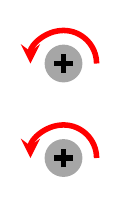
\begin{tikzpicture}
				\tikzset{
					textDef/.style={font=\sffamily\small,},
					lineScaled/.style={line width={4pt}},
					arrowStyle/.style={line width={2pt}, >=stealth, red},
				}
				\mikrotikInsideEnclosure{0.5}{0}{0}{0}
				\mikrotikGatewayTopEnclosure{0.5}{0}{0}{0}
				
				\begin{scope}[shift={(0, -1.7)}, scale=0.6]
					\fill[gray!70] (0, 0) circle (4mm);
					\draw[black, line width=2pt] (-0.2, 0) -- (0.2, 0);
					\draw[black, line width=2pt] (0, -0.2) -- (0, 0.2);
					\draw[->, arrowStyle] (0:7mm) arc (0:180:7mm);
				\end{scope}
				
				\begin{scope}[shift={(0, -2.9)}, scale=0.6]
					\fill[gray!70] (0, 0) circle (4mm);
					\draw[black, line width=2pt] (-0.2, 0) -- (0.2, 0);
					\draw[black, line width=2pt] (0, -0.2) -- (0, 0.2);
					\draw[->, arrowStyle] (0:7mm) arc (0:180:7mm);
				\end{scope}
			\end{tikzpicture}
			\caption{Entfernen der Schrauben}
		\end{figure}
	
	
		\begin{figure}[H]
			\centering
			\begin{tikzpicture}
				\tikzset{
					textDef/.style={font=\sffamily\small,},
					lineScaled/.style={line width={4pt}},
					lineDef/.style={line width={2pt}},
					arrowStyle/.style={line width={2pt}, >=stealth, red},
				}
				\mikrotikInsideEnclosure{0.5}{0}{0}{0}
				\routerPlatform{0.5}{90}{0}{1.9}
				\loraCard{0.5}{90}{0}{1.9}
				\draw[lineDef, black] (SMA-INPUT) -- ++(0, 0.5) -- ++(0.2, 0.2) -- ++(0, 1.5) -- (CARD-UFL-CONNECTOR) node[circle, fill=Gold, inner sep=2.5pt] {};
				
				\mikrotikGatewayTopEnclosure{0.5}{0}{0}{2.5}
				
				\draw[arrowStyle, <-] ($(SMA-OUTPUT) + (2, 0)$) -- ++(0,1);
				
			\end{tikzpicture}
			\caption{Innenteil aus dem Gehäuse herausziehen}
		\end{figure}

	\subsection{Ersteinrichtung}
	\textcite{mikrotik:2025z} beschreibt die Ersteinrichtung des Geräts wie folgt:
	
	\begin{enumerate}
		\item Stelle sicher, dass dein Internetanbieter einen Gerätewechsel zulässt und automatisch eine IP-Adresse vergibt.
		\item Öffne die untere Abdeckung des Geräts.
		\item Schlie{\ss}e eine externe Antenne an den SMA-Anschluss an.
		\item Verbinde das Gerät mit der Stromversorgung.
		\item Verbinde dich mit dem MikroTik-WLAN des Geräts.
		\item Führe die Konfiguration über das WLAN mithilfe eines Webbrowsers.
		\item Alternativ kann das Konfigurationswerkzeug WinBox verwendet werden; 
		standardmä{\ss}ig ist der Zugriff über den Ethernet-Port jedoch durch die Firewall blockiert.
		\item Öffne nach der WLAN-Verbindung die Adresse 
		\url{http://192.168.88.1}, um mit der Konfiguration zu beginnen.
		\item Melde dich an: Benutzername \textbf{admin}, kein Standardpasswort.
		\item Wähle in der mobilen App „Quick setup“, um durch den sechs­stufigen Einrichtungsprozess geführt zu werden.
		\item Finde die Gateway-ID auf dem Geräteetikett und registriere sie in deinem Network Server.
		\item Um das Gerät mit dem LoRa Network Server zu verbinden, siehe \autoref{mikrotik:connectToLns}
		\item Klicke auf „Check for updates“ und aktualisiere RouterOS auf die neueste Version (erfordert aktive Internetverbindung).
		\item Wähle anschlie{\ss}end das Land aus, um die jeweiligen regulatorischen Vorgaben zu aktivieren.
		\item Lege ein WLAN-Passwort fest.
		\item Setze das Router-Administratorpasswort.
	\end{enumerate}
	
	
	
	\subsection{Anbinden an \acl{lns} \label{mikrotik:connectToLns}}
	
		\textbf{Voraussetzung:} Das Gateway ist per LAN-Kabel mit dem Netzwerk verbunden und die korrekte Antenne ist angeschlossen. Die Konfiguration kann von jedem Gerät im selben Netzwerk durchgeführt werden, sofern die Zugangsdaten des Gateways bekannt sind. Zudem muss ein LoRaWAN-Server vorhanden sein, dessen IP-Adresse für die spätere Anbindung benötigt wird. Für die Demonstration wird die Server-IP \PYTHON{192.168.0.102} verwendet.
		
		
		\begin{enumerate}
			\item \textbf{Anmeldung am Gateway}  \\
			Zur Anmeldung am Gateway wird dessen IP-Adresse benötigt, da über sie der Zugriff auf die Konfigurationsoberfläche erfolgt. Im Beispiel lautet sie \PYTHON{192.168.8.4}. Die IP-Adresse kann im \textit{Clients Table} des Routers oder mithilfe von Tools wie \textit{LanScan} ermittelt werden.  
			Die IP-Adresse wird anschlie{\ss}end in die Adresszeile des Webbrowsers eingetragen. Das Gerät, von dem aus die Konfiguration vorgenommen wird, muss sich im selben LAN wie das Gateway befinden \cite{mikrotik:2020}, \cite{mikrotik:2024b}.
			
			
			
			Bei der Anmeldung werden der während der Erstkonfiguration vergebene \textbf{Benutzername} und das \textbf{Passwort} benötigt.
			
			\begin{figure}[H]
				\centering
				\begin{tikzpicture}
					\tikzset{
						textDef/.style={font=\sffamily\small,},
						lineScaled/.style={line width={2pt}},
						arrowStyle/.style={lineScaled, >=stealth, red},
					}
					\node[anchor=south west, inner sep=0] (image) at (0,0) {%
						
\includegraphics[width=0.8\linewidth]{LoRaAndLoRaWAN/Gateway/MikrotikGUI}};
					
					\begin{scope}[x={(image.south east)}, y={(image.north west)}]
						\draw[arrowStyle, <-] (0.5, 0.935) -- ++(0,-0.1) node[textDef, below] {1};
						\draw[arrowStyle, <-] (0.38, 0.52) -- ++(0.1,0.02) node[textDef, right] {2};
						\draw[arrowStyle, <-] (0.38, 0.48) -- ++(0.1,-0.02) node[textDef, right] {3};
					\end{scope}
				\end{tikzpicture}
				\caption{Eingabe der neuen Zugangsdaten}
			\end{figure}
			
			Nach Eingabe der Daten wird die Anmeldung mit der entsprechenden Schaltfläche bestätigt.
		
		
		\item \textbf{Hinzufügen eines neuen Servers}  \\
		Nach dem Login wird über die Schaltfläche \textit{WebFig} (\textbf{1}) die grafische Oberfläche geöffnet. Unter dem Menüpunkt \textit{IoT} (\textbf{2}) befindet sich der Bereich \textit{LoRa} (\textbf{3}); dort wird der Reiter \textit{Server} (\textbf{4}) ausgewählt.
		
		\begin{figure}[H]
			\centering
			\begin{tikzpicture}
				\tikzset{
					textDef/.style={font=\sffamily\small,},
					lineScaled/.style={line width={2pt}},
					arrowStyle/.style={lineScaled, >=stealth, red},
				}
				\node[anchor=south west, inner sep=0] (image) at (0,0) {%
					
\includegraphics[width=0.8\linewidth]{LoRaAndLoRaWAN/Gateway/MikrotikAddServer}};
				
				\begin{scope}[x={(image.south east)}, y={(image.north west)}]
					\draw[arrowStyle, <-] (0.81, 0.865) -- ++(0,-0.07) node[textDef, below] {1};
					\draw[arrowStyle, <-] (0.1, 0.365) -- ++(0.07,0.02) node[textDef, right] {2};
					\draw[arrowStyle, <-] (0.1, 0.305) -- ++(0.07,-0.02) node[textDef, right] {3};
					\draw[arrowStyle, <-] (0.35, 0.81) -- ++(0,-0.07) node[textDef, below] {4};
				\end{scope}
			\end{tikzpicture}
			\caption{Navigieren zum Server-Menü}
		\end{figure}
		
		Hier wird eine Liste vorkonfigurierter Server angezeigt.
		
		\begin{figure}[H]
			\centering
			\begin{tikzpicture}
				\tikzset{
					textDef/.style={font=\sffamily\small,},
					lineScaled/.style={line width={2pt}},
					arrowStyle/.style={lineScaled, >=stealth, red},
					boxStyle/.style={line width={1pt}, red},
				}
				\node[anchor=south west, inner sep=0] (image) at (0,0) {%
					
\includegraphics[width=0.8\linewidth]{LoRaAndLoRaWAN/Gateway/MikrotikAddServer}};
				
				\begin{scope}[x={(image.south east)}, y={(image.north west)}]
					\draw[boxStyle] (0.2, 0.31) rectangle ++(0.7, 0.4);
				\end{scope}
			\end{tikzpicture}
			\caption{Liste der vorkonfigurierten Server}
		\end{figure}
		
		Soll ein neuer Server hinzugefügt werden, wird die Schaltfläche \textit{Add New} ausgewählt.
		
		\begin{figure}[H]
			\centering
			\begin{tikzpicture}
				\tikzset{
					textDef/.style={font=\sffamily\small,},
					lineScaled/.style={line width={2pt}},
					arrowStyle/.style={lineScaled, >=stealth, red},
				}
				\node[anchor=south west, inner sep=0] (image) at (0,0) {%
					
\includegraphics[width=0.8\linewidth]{LoRaAndLoRaWAN/Gateway/MikrotikAddServer}};
				
				\begin{scope}[x={(image.south east)}, y={(image.north west)}]
					\draw[arrowStyle, <-] (0.205, 0.765) -- ++(0.1,0);
				\end{scope}
			\end{tikzpicture}
			\caption{Hinzufügen eines neuen Servers}
		\end{figure}
		
		Im nächsten Schritt werden die Serverdaten eingetragen:  
		Ein frei wählbarer Name, die IP-Adresse des \ac{lns} (in der Regel die IP-Adresse der \ac{lns}-Hostmaschine, im Beispiel \PYTHON{192.168.8.102}), das verwendete Protokoll (UDP) sowie die Standardports für das UDP-Protokoll (1700) müssen eingetragen werden. Anschlie{\ss}end werden die Angaben mit \textit{OK} bestätigt.
		
		
		\begin{figure}[H]
			\centering
			\begin{tikzpicture}
				\tikzset{
					textDef/.style={font=\sffamily\small,},
					lineScaled/.style={line width={2pt}},
					arrowStyle/.style={lineScaled, >=stealth, red},
					boxStyle/.style={line width={1pt}, red},
				}
				\node[anchor=south west, inner sep=0] (image) at (0,0) {%
					
\includegraphics[width=0.8\linewidth]{LoRaAndLoRaWAN/Gateway/MikrotikServerData}};
				
				\begin{scope}[x={(image.south east)}, y={(image.north west)}]
					\draw[boxStyle] (0.25, 0.5) rectangle ++(0.27, 0.27);
					\draw[arrowStyle, <-] (0.83, 0.40) -- ++(0,0.1);
				\end{scope}
			\end{tikzpicture}
			\caption{Eingabe der Serverdaten}
		\end{figure}
		
		\item \textbf{Zuordnen des Gateways zum neuen Server}  
		Zunächst muss das Gateway dem neuen Server zugewiesen werden. Dazu wird die Schaltfläche \textit{Devices} geöffnet (\textbf{1}) und anschlie{\ss}end das gewünschte Gateway ausgewählt (\textbf{2}).
		
		\begin{figure}[H]
			\centering
			\begin{tikzpicture}
				\tikzset{
					textDef/.style={font=\sffamily\small,},
					lineScaled/.style={line width={2pt}},
					arrowStyle/.style={lineScaled, >=stealth, red},
				}
				\node[anchor=south west, inner sep=0] (image) at (0,0) {%
					
\includegraphics[width=0.8\linewidth]{LoRaAndLoRaWAN/Gateway/MikrotikDevices}};
				
				\begin{scope}[x={(image.south east)}, y={(image.north west)}]
					\draw[arrowStyle, <-] (0.17, 0.81) -- ++(0,-0.1) node[textDef, below] {1};
					\draw[arrowStyle, <-] (0.53, 0.62) -- ++(0.05,-0.1) node[textDef, below] {2};
				\end{scope}
			\end{tikzpicture}
			\caption{Auswahl des Gateways}
		\end{figure}
		
		\item \textbf{Ändern der Geräteeinstellungen}\\
		Um die Geräteeinstellungen anpassen zu können, muss das Gerät zunächst deaktiviert werden. Dies geschieht über die Schaltfläche \textit{Enable} (\textbf{1}), die deaktiviert wird, und anschlie{\ss}end durch Bestätigen mit \textit{Apply} (\textbf{2}).
		
		\begin{figure}[H]
			\centering
			\begin{tikzpicture}
				\tikzset{
					textDef/.style={font=\sffamily\small,},
					lineScaled/.style={line width={2pt}},
					arrowStyle/.style={lineScaled, >=stealth, red},
				}
				\node[anchor=south west, inner sep=0] (image) at (0,0) {%
					
\includegraphics[width=0.8\linewidth]{LoRaAndLoRaWAN/Gateway/DeviceSettings}};
				
				\begin{scope}[x={(image.south east)}, y={(image.north west)}]
					\draw[arrowStyle, <-] (0.395, 0.7325) -- ++(0.1,0) node[textDef, right] {1};
					\draw[arrowStyle, <-] (0.785, 0.08) -- ++(0,0.1) node[textDef, above] {2};
				\end{scope}
			\end{tikzpicture}
			\caption{Deaktivieren des Geräts}
		\end{figure}
		
		Nun können die Einstellungen angepasst werden. Ein frei wählbarer Name kann vergeben werden (\textbf{1}). Die \PYTHON{Gateway EUI} (\textbf{2}) sollte notiert werden, da sie später für die Konfiguration des \ac{lns} benötigt wird.  
		Unter der Liste \textit{Network Servers} (\textbf{3}) wird der zuvor konfigurierte Server ausgewählt. Zusätzlich muss sichergestellt werden, dass der \textit{Channel Plan} (\textbf{4}) dem in der EU zulässigen Plan entspricht.  
		Au{\ss}erdem muss die Sendeleistung der angeschlossenen Antenne angegeben werden (\textbf{5}), unter Berücksichtigung der Kabelverluste \cite{mikrotik:2024b}.  
		Abschlie{\ss}end werden die Änderungen mit der Schaltfläche \textit{Apply} (\textbf{6}) übernommen.
		
		
		\begin{figure}[H]
			\centering
			\begin{tikzpicture}
				\tikzset{
					textDef/.style={font=\sffamily\small,},
					lineScaled/.style={line width={2pt}},
					arrowStyle/.style={lineScaled, >=stealth, red},
				}
				\node[anchor=south west, inner sep=0] (image) at (0,0) {%
					
\includegraphics[width=0.8\linewidth]{LoRaAndLoRaWAN/Gateway/MikrotikChangeDevSettings}};
				
				\begin{scope}[x={(image.south east)}, y={(image.north west)}]
					\draw[arrowStyle, <-] (0.5, 0.59) -- ++(0.1,0.01) node[textDef, right] {1};
					\draw[arrowStyle, <-] (0.5, 0.54) -- ++(0.1,-0.01) node[textDef, right] {2};
					\draw[arrowStyle, <-] (0.5, 0.45) -- ++(0.1,0.01) node[textDef, right] {3};
					\draw[arrowStyle, <-] (0.5, 0.40) -- ++(0.1,-0.01) node[textDef, right] {4};
					\draw[arrowStyle, <-] (0.5, 0.35) -- ++(0.1,-0.015) node[textDef, right] {5};
					\draw[arrowStyle, <-] (0.785, 0.08) -- ++(0,0.1) node[textDef, above] {6};
				\end{scope}
			\end{tikzpicture}
			\caption{Anpassen der Geräteeinstellungen}
		\end{figure}
		
		Nach Abschluss der Änderungen muss das Gateway wieder aktiviert werden, indem die Schaltfläche \textit{Enable} aktiviert und anschlie{\ss}end mit \textit{Apply} bestätigt wird.  
		Nun ist das Gateway bereit, mit dem \ac{lns} verbunden zu werden (siehe Einleitung zum jeweiligen \ac{lns}).
		
		

	\end{enumerate}


